\documentclass[11pt]{amsart}
\usepackage[utf8]{inputenc}
\usepackage{amsmath,amssymb,amsthm}
\usepackage{enumitem}
\usepackage{geometry}
\usepackage{tikz,forest}
\usetikzlibrary{arrows.meta} 
\geometry{margin=1.1in}
% --- theorem-like environments ------------------------------------
\usepackage{amsthm}           % already present in most maths templates
\newtheorem{theorem}{Theorem}[section]   % numbered within sections
\newtheorem{lemma}[theorem]{Lemma}
\newtheorem{corollary}[theorem]{Corollary}
\theoremstyle{remark}            % estilo sem itálico, como Observações
\newtheorem{remark}[theorem]{Remark}  
\usepackage{graphicx}   % habilita \includegraphics
\usepackage{caption}    % (opcional) controla formatação de legendas
% ------------------------------------------------------------------

\title{Manual for the Structure \texttt{BinaryTreeWithRootandTops}}
\author{}
\date{}

\newcommand{\pairToFinset}{\mathsf{pairToFinset}}
\newcommand{\supp}{\mathsf{Combinatorial\_Support}}
\newcommand{\Fin}{\mathsf{Finset}}

\begin{document}
\maketitle

 

\section{Structure \texttt{BinaryTreeWithRootandTops}}


\subsection{Notation}
Given a Pair $p=(p.1,p.2)$, we have 
\begin{itemize}[leftmargin=1.5em]
  \item $\Fin\alpha$ denotes a \emph{finite} subset of $\alpha$ (Lean’s \texttt{Finset}).
  \item Given $p : \Fin\alpha\times\Fin\alpha$,  
        $\pairToFinset(p) \;=\; \{ p.1, p.2\}$.
        \begin{figure}[h]             % floating environment (optional but recommended)
  \centering                     % centre the graphic
  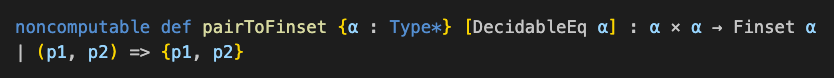
\includegraphics[width=0.99\linewidth]{pairfinset.png} % ← path + scaling option
\end{figure}
  \item $\supp(p)= p.1\cup p.2$ is the “combinatorial support’’  
       \begin{figure}[h]             % floating environment (optional but recommended)
  \centering                     % centre the graphic
  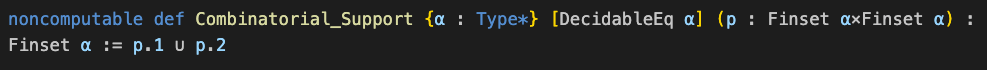
\includegraphics[width=0.99\linewidth]{combsup.png} % ← path + scaling option
\end{figure}
  \item \textbf{Disjoint}$(A,B)$ abbreviates $A\cap B=\varnothing$.
\end{itemize}

\subsection{Overview}






\textbf{Data.}  The record 
\[
\texttt{BinaryTreeWithRootandTops}
\bigl(\alpha : \mathrm{Type}^\ast\bigr)
\quad [\mathrm{DecidableEq}\,\alpha]
\]
stores four finite objects:

\begin{itemize}[leftmargin=1.8em]
  \item \textbf{Childs} : $\Fin \alpha$ — the ground set (assumed non-empty);
  \item \textbf{Root}   : $\Fin\alpha \times \Fin\alpha$ — the first split of \textbf{Childs};
  \item \textbf{Branches} : $\Fin\bigl(\Fin\alpha \times \Fin\alpha\bigr)$ —
        all interior nodes, including \textbf{Root};
  \item \textbf{Tops}   : $\Fin \alpha$ — the labels of distinguished leaves.
\end{itemize}
 
\paragraph{Laminar family of supports.}
The supports of the branches satisfy two crucial axioms:

\begin{enumerate}[label=\textbf{(L\arabic*)},leftmargin=1.8em]
  \item \emph{Cover.}  $\displaystyle
        \bigcup_{p\in\textbf{Branches}} \supp(p) \;=\; \textbf{Childs}.$
  \item \emph{Nesting.}  Whenever $p\neq q$ in \textbf{Branches},
        the supports are either disjoint or properly nested:
       \begin{align*} 
        \supp(p)\cap\supp(q)=\varnothing
        \quad\text{or}\\ \quad
        \supp(p)\subseteq\supp(q)
        \quad\text{or}\\\quad
        \supp(q)\subseteq\supp(p).
        \end{align*} 
\end{enumerate}

Indeed something even stronger happens, the family 
$$
\mathcal{L}\;=\;\{p.1, p.2 \mid p\in\textbf{Branches}\}
$$
is a \emph{maximal laminar family} (nested set system) on \textbf{Childs}.  
The record not only remembers this hierarchy of blocks but also keeps track of
\emph{how each block is split}: for every non-leaf support
$S\in\mathcal{L}$ there exists \emph{at most  one} ordered pair
$(A,B)\in\textbf{Branches}$ with $A\cup B=S$, $A\cap B=\varnothing$ and
$\supp(A,B)=S$.  This extra orientation (left vs.\ right child) upgrades the
laminar family into a full binary tree.

Singleton supports $\{t\}$ correspond precisely to the leaf pairs
$(\{t\},\{\,\})$ or $(\{\,\},\{t\})$; the set of all such labels is stored in
the field \textbf{Tops}.
% -----------------------------------------------------------

 

\subsection{Fields}

\begin{description}[style=unboxed,leftmargin=0pt]

\item[\textbf{\texttt{Root} : $\Fin\alpha\times\Fin\alpha$}]  
  The distinguished ordered pair that serves as the root of the tree.

\item[\textbf{\texttt{Childs} : $\Fin\alpha$}]  
  The finite set of all basic symbols that may appear in either component of a branch pair.

\item[\textbf{\texttt{Branches} : $\Fin(\Fin\alpha\times\Fin\alpha)$}]  
  The finite family of  ordered pairs that form the vertices of the tree,
  including \texttt{Root}.

\item[\textbf{\texttt{Tops} : $\Fin\alpha$}]  
  A specified finite subset of~\texttt{Childs} whose singletons appear as leaf pairs.

\end{description}

\subsection{Structure properties}

All quantifiers range over the corresponding finite sets declared above.

\begin{enumerate}[label=\textbf{(\arabic*)},leftmargin=1.5em]
  \item \textbf{Non-empty components.}\\
        $\forall\,y\in\texttt{Branches},\; y.1\neq\varnothing\; \land\; y.2\neq\varnothing$.

  \item \textbf{Disjoint components.}\\
        $\forall\,p\in\texttt{Branches},\; p.1\cap p.2 = \varnothing$.

  \item \textbf{Distinct pairs are disjoint as sets.}\\
        $\forall\,p,q\in\texttt{Branches},\; p\neq q \;\to\;
        \bigl(\pairToFinset(p)\bigr)\cap\bigl(\pairToFinset(q)\bigr)=\varnothing$.

  \item \textbf{Root belongs to the branch set.}\\
        $\texttt{Root}\in\texttt{Branches}$.

  \item \textbf{Every child occurs in some branch.}\\
        $\forall\,a\in\texttt{Childs},\;\exists\,p\in\texttt{Branches},\;
        a\in\supp(p)$.

  \item \textbf{Children are contained in the root pair.}\\
        $\texttt{Childs}\subseteq\texttt{Root}.1\cup\texttt{Root}.2$.

  \item \textbf{Branch components are made of children.}\\
        $\forall\,p\in\texttt{Branches},\;
        p.1\subseteq\texttt{Childs}\;\land\; p.2\subseteq\texttt{Childs}$.

  \item \textbf{Recursive tree structure.}\\
        $\forall\,p\in\texttt{Branches},\; p\neq\texttt{Root}\;
        \to\; \exists\,q\in\texttt{Branches},\;
        p.1\cup p.2 \in \pairToFinset(q)$.

  \item \textbf{Tops are witnessed by singleton pairs.}\\
        $\forall\,t\in\texttt{Tops},\;\exists\,q\in\texttt{Branches},\;
        \{t\}\in\pairToFinset(q)$.

  \item \textbf{Singletons in any branch are tops.}\\
        $\forall\,p\in\texttt{Branches},\;
        \forall\,x,\; \{x\}\in\pairToFinset(p)\;\to\; x\in\texttt{Tops}$.

  \item \textbf{Non-empty root and child set.}\\
        $\texttt{Root}.1\neq\varnothing,\;
        \texttt{Root}.2\neq\varnothing,\;
        \texttt{Childs}\neq\varnothing$.

  \item \textbf{Root components are disjoint.}\\
        $\texttt{Root}.1\cap\texttt{Root}.2=\varnothing$.

  \item \textbf{Support property (tree compatibility).}\\
      \begin{align*} \forall\,p,q\in\texttt{Branches},\; p\neq q\;\to \\
        \bigl(\, \supp(p)\cap\supp(q)=\varnothing\;\bigl)\;\lor\; \\ 
        \supp(p)\subseteq q.1\;\lor\;\supp(p)\subseteq q.2\;\lor\; \\
        \supp(q)\subseteq p.1\;\lor\;\supp(q)\subseteq p.2.
   \end{align*} 
\end{enumerate}
\newpage 
\begin{figure}[t]             % floating environment (optional but recommended)
  \centering                     % centre the graphic
  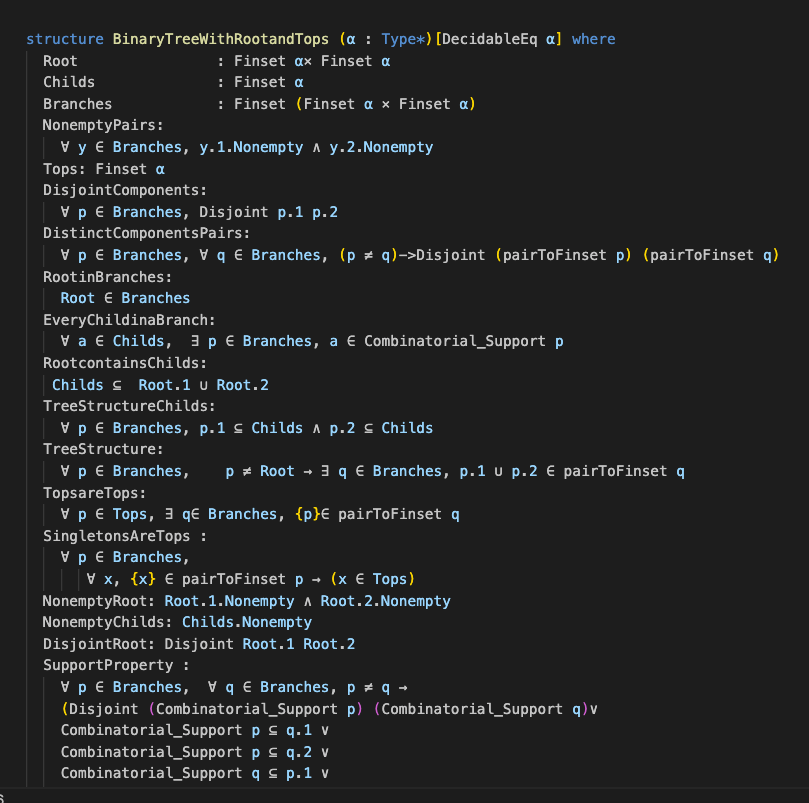
\includegraphics[width=0.99\linewidth]{tree.png} % ← path + scaling option
\end{figure}


\subsection{Example}

Let
\[
\begin{aligned}
\texttt{Childs} \; &= \; \{1,2,3,4,5,6,7\}, \\[4pt]
\texttt{Root} \; &= \; (\{1,2,3\},\; \{4,5,6,7\}), \\[4pt]
\texttt{Branches} \; &= \;
\bigl\{
  (\{1,2,3\},\{4,5,6,7\}),\;
  (\{1,2\},\{3\}),\;
  (\{4,5\},\{6,7\}), \\[-2pt]
  &\hphantom{=\bigl\{}
 \;
  (\{4\},\{5\}),\;
  (\{6\},\{7\})
\bigr\}, \\[4pt]
\text{Tops} \; &= \; \{3,4,6,7\}.
\end{aligned}
\]
and we can see the tree structure graphically below \\

\begin{forest}
for tree = {
  rectangle, rounded corners, draw,
  align=center,          % centre each label
  minimum width=16mm,    % uniform node size (adjust to taste)
  s sep=7mm,             % vertical separation
  l sep=8mm,            % horizontal separation
  edge+={-{Stealth[]}},  % arrows parent→child
  font=\small
}
% ---------------------- tree specification -------------------------
[{$\texttt{Childs} = \{1,2,3,4,5,6,7\}$}
[{$\texttt{Root} = (\{1,2,3\},\{4,5,6,7\})$ \\ $\in \texttt{Branches}$}         % ← Root
  [{$(\{1,2\},\{3\}) $ \\ $\in \texttt{Branches}$}               % first split of left block
    [{$3$ \\ $\in \texttt{Tops}$}]    % singleton leaf = top
  ]
  [{$(\{4,5\},\{6,7\})$ \\ $\in \texttt{Branches}$ }             % first split of right block
    [{$(\{4\},\{5\})  $ \\ $\in \texttt{Branches}$}
      [{$4$ \\ $\in \texttt{Tops}$}]
      [{$5$ \\ $\in \texttt{Tops}$}]
    ]
    [{$(\{6\},\{7\}) $ \\ $\in \texttt{Branches}$}
      [{$6$ \\ $\in \texttt{Tops}$}]
      [{$7$ \\ $\in \texttt{Tops}$}]
    ]
  ]
]
]
\end{forest}

% -----------------------------------------------------------
% 6.  Main Results
% -----------------------------------------------------------
\section*{Main Result}

\begin{theorem}[\texttt{exists\_tree\_childs\_eq\_C\_and\_all\_childs\_in\_Tops\_of\_card\_ge\_two}
] Let  $C$ be a finite set with at least two elements. Then there exists a structure
\[
T \;:\; \texttt{BinaryTreeWithRootandTops} 
\]
such that
\[
T.\texttt{Childs}=C
\quad\text{and}\quad
T.\texttt{Tops}=C.
\]
\begin{figure}[htbp]             % floating environment (optional but recommended)
  \centering                     % centre the graphic
  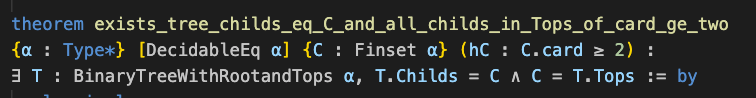
\includegraphics[width=0.99\linewidth]{main.png} % ← path + scaling option
\end{figure}
\end{theorem}


\subsection{Example} In the  previous example we do not have $T.Tops=T.Childs$, however we can complete it as 

\begin{forest}
for tree = {
  rectangle, rounded corners, draw,
  align=center,          % centre each label
  minimum width=16mm,    % uniform node size (adjust to taste)
  s sep=7mm,             % vertical separation
  l sep=8mm,            % horizontal separation
  edge+={-{Stealth[]}},  % arrows parent→child
  font=\small
}
% ---------------------- tree specification -------------------------
[{$\texttt{Childs} = \{1,2,3,4,5,6,7\}$}
[{$\texttt{Root} = (\{1,2,3\},\{4,5,6,7\})$ \\ $\in \texttt{Branches}$}         % ← Root
  [{$(\{1,2\},\{3\})$ \\ $\in \texttt{Branches}$}               % first split of left block
    [{$(\{1\},\{2\}) $ \\ $\in \texttt{Branches}$}
      [{$1$ \\ $\in \texttt{Tops}$}]
      [{$2$ \\ $\in \texttt{Tops}$}]
    ]  
    [{$3$ \\ $\in \texttt{Tops}$}]    % singleton leaf = top
  ]
  [{$(\{4,5\},\{6,7\})$ \\ $\in \texttt{Branches}$ }             % first split of right block
    [{$(\{4\},\{5\})  $ \\ $\in \texttt{Branches}$}
      [{$4$ \\ $\in \texttt{Tops}$}]
      [{$5$ \\ $\in \texttt{Tops}$}]
    ]
    [{$(\{6\},\{7\}) $ \\ $\in \texttt{Branches}$}
      [{$6$ \\ $\in \texttt{Tops}$}]
      [{$7$ \\ $\in \texttt{Tops}$}]
    ]
  ]
]
]
\end{forest}




 
\end{document}
